% Options for packages loaded elsewhere
\PassOptionsToPackage{unicode}{hyperref}
\PassOptionsToPackage{hyphens}{url}
%
\documentclass[
]{report}
\title{Econometrics vizualisation}
\author{Lucas Chaveneau, Thibault Fuchez, Allan Guichard}
\date{2021-11-04}

\usepackage{amsmath,amssymb}
\usepackage{lmodern}
\usepackage{iftex}
\ifPDFTeX
  \usepackage[T1]{fontenc}
  \usepackage[utf8]{inputenc}
  \usepackage{textcomp} % provide euro and other symbols
\else % if luatex or xetex
  \usepackage{unicode-math}
  \defaultfontfeatures{Scale=MatchLowercase}
  \defaultfontfeatures[\rmfamily]{Ligatures=TeX,Scale=1}
\fi
% Use upquote if available, for straight quotes in verbatim environments
\IfFileExists{upquote.sty}{\usepackage{upquote}}{}
\IfFileExists{microtype.sty}{% use microtype if available
  \usepackage[]{microtype}
  \UseMicrotypeSet[protrusion]{basicmath} % disable protrusion for tt fonts
}{}
\makeatletter
\@ifundefined{KOMAClassName}{% if non-KOMA class
  \IfFileExists{parskip.sty}{%
    \usepackage{parskip}
  }{% else
    \setlength{\parindent}{0pt}
    \setlength{\parskip}{6pt plus 2pt minus 1pt}}
}{% if KOMA class
  \KOMAoptions{parskip=half}}
\makeatother
\usepackage{xcolor}
\IfFileExists{xurl.sty}{\usepackage{xurl}}{} % add URL line breaks if available
\IfFileExists{bookmark.sty}{\usepackage{bookmark}}{\usepackage{hyperref}}
\hypersetup{
  pdftitle={Econometrics vizualisation},
  pdfauthor={Lucas Chaveneau, Thibault Fuchez, Allan Guichard},
  hidelinks,
  pdfcreator={LaTeX via pandoc}}
\urlstyle{same} % disable monospaced font for URLs
\usepackage{longtable,booktabs,array}
\usepackage{calc} % for calculating minipage widths
% Correct order of tables after \paragraph or \subparagraph
\usepackage{etoolbox}
\makeatletter
\patchcmd\longtable{\par}{\if@noskipsec\mbox{}\fi\par}{}{}
\makeatother
% Allow footnotes in longtable head/foot
\IfFileExists{footnotehyper.sty}{\usepackage{footnotehyper}}{\usepackage{footnote}}
\makesavenoteenv{longtable}
\usepackage{graphicx}
\makeatletter
\def\maxwidth{\ifdim\Gin@nat@width>\linewidth\linewidth\else\Gin@nat@width\fi}
\def\maxheight{\ifdim\Gin@nat@height>\textheight\textheight\else\Gin@nat@height\fi}
\makeatother
% Scale images if necessary, so that they will not overflow the page
% margins by default, and it is still possible to overwrite the defaults
% using explicit options in \includegraphics[width, height, ...]{}
\setkeys{Gin}{width=\maxwidth,height=\maxheight,keepaspectratio}
% Set default figure placement to htbp
\makeatletter
\def\fps@figure{htbp}
\makeatother
\setlength{\emergencystretch}{3em} % prevent overfull lines
\providecommand{\tightlist}{%
  \setlength{\itemsep}{0pt}\setlength{\parskip}{0pt}}
\setcounter{secnumdepth}{5}
\usepackage{booktabs}
\ifLuaTeX
  \usepackage{selnolig}  % disable illegal ligatures
\fi
\usepackage[]{natbib}
\bibliographystyle{apalike}

\begin{document}
\maketitle

{
\setcounter{tocdepth}{1}
\tableofcontents
}
\hypertarget{introduction}{%
\chapter{Introduction}\label{introduction}}

Nous avons comme projet de proposer une librairie développé sous R qui propose différents moyens de visualiser les éléments essentiels de l'économètre.

L'économétrie est une branche de la science économique qui a pour but de d'estimer et de tester les modèles économiques (représentation simplifiée de la réalité). Ainsi l'économètre essaie d'identifier les paramètres d'un modèle à l'aide d'estimation statistique, il cherche donc à induire les caractéristiques d'un groupe général (la population) à partir de celles d'un groupe particulier (l'échantillon).

Trois mots essentiels dans le langage de l'économètre sont: la corrélation, la regression, et la causalité.

Afin de mieux comprendre les liens entres différentes variables, la visualisation est un outil clé qui aide à interpréter les résultats mathématiques et statistiques.

Notre package s'intéressera donc à la représentation des corrélations. Nous essaierons de mettre en avant une représentation claire et synthétique de la covariance, ainsi qu'une représentation des éléments qui permettent de visualiser la qualité d'une regression ainsi que la part de chaque variable dans l'explication de la variable à prédire.

Ce document a pour vocation d'accompagner le package. Il propose une définition des outils économétrique nécessaires à la compréhension du package. Il propose également un état des lieux des différentes techniques de visualisation qui existent déjà.

\hypertarget{la-covariance}{%
\chapter{La covariance}\label{la-covariance}}

\hypertarget{rappel-de-la-duxe9finition-de-la-variance}{%
\section{Rappel de la définition de la variance :}\label{rappel-de-la-duxe9finition-de-la-variance}}

En statistique et en théorie des probabilités, la variance est une mesure de la dispersion des valeurs d'un échantillon ou d'une distribution de probabilité. Elle exprime la moyenne des carrés des écarts à la moyenne, aussi égale à la différence entre la moyenne des carrés des valeurs de la variable et le carré de la moyenne, selon le théorème de König-Huygens.

\begin{itemize}
\tightlist
\item
  Classical formula of variance :
\end{itemize}

\[\sigma^2_x=\frac{1}{n}\sum_{x=1}^{n}(x_i - \bar{x})^2 = \frac{1}{n}\sum_{x=1}^{n}x_i^2 - \bar{x}^2 \]

\begin{itemize}
\tightlist
\item
  A new proposition for variance formula\citep{Heffernan}:
\end{itemize}

\[\sigma^2_x= \frac{1}{n(n-1)}\sum_{i=1}^{n-1}\sum_{j>i}^{n}(x_i-x_j)^2\]

\begin{itemize}
\tightlist
\item
  Variance vs.~Covariance:
\end{itemize}

Variance and covariance are mathematical terms frequently used in statistics and probability theory. Variance refers to the spread of a data set around its mean value, while a covariance refers to the measure of the directional relationship between two random variables.

\hypertarget{duxe9finition-littuxe9raire-usuelle-de-la-covariance}{%
\section{Définition littéraire usuelle de la covariance}\label{duxe9finition-littuxe9raire-usuelle-de-la-covariance}}

``A covariance refers to the measure of how two random variables will change when they are compared to each other.''

La covariance est une extension de la notion de variance. La covariance entre deux variables aléatoires est un nombre permettant de quantifier leurs écarts conjoints par rapport à leurs espérances respectives.

Intuitivement, la covariance est une mesure de la variation simultanée de deux variables aléatoires. C'est-à-dire que la covariance devient plus positive pour chaque couple de valeurs qui diffèrent de leur moyenne dans le même sens, et plus négative pour chaque couple de valeurs qui diffèrent de leur moyenne dans le sens opposé.

La covariance de deux variables aléatoires indépendantes est nulle, bien que la réciproque ne soit pas toujours vraie.

Ce concept se généralise naturellement à plusieurs variables (vecteur aléatoire) par la matrice de covariance (ou matrice de variance-covariance) qui, pour un ensemble de p variables aléatoires réelles \(X_1\), etc.,\(Xp\) est la matrice carrée dont l'élément de la ligne i et de la colonne j est la covariance des variables \(X_i\) et \(X_j\). Cette matrice permet de quantifier la variation de chaque variable par rapport à chacune des autres.

``The sign of the covariance therefore shows the tendency in the linear relationship between the variables. The magnitude of the covariance is not easy to interpret because it is not normalized and hence depends on the magnitudes of the variables''.

\hypertarget{duxe9finitions-mathuxe9matique-usuelle-et-alternatives}{%
\section{Définitions mathématique usuelle et alternatives}\label{duxe9finitions-mathuxe9matique-usuelle-et-alternatives}}

\begin{itemize}
\tightlist
\item
  covariance formula :
\end{itemize}

\[cov(X,Y) = \frac{1}{n-1}\sum_{i=1}^{n}(x_i - \bar{x})(y_i - \bar{y}) \]

\begin{itemize}
\tightlist
\item
  formula from heffernan definition of covariance :
\end{itemize}

\[cov(X,Y)= \frac{2}{n(n-1)}\sum_{i=1}^{n-1}\sum_{j>i}^{n}\frac{1}{2}(x_i-x_j)(y_i - y_j)\]

\begin{itemize}
\tightlist
\item
  lister autres \ldots{}
\end{itemize}

\hypertarget{la-corruxe9lation}{%
\chapter{La corrélation}\label{la-corruxe9lation}}

\hypertarget{de-la-covariance-uxe0-la-corruxe9lation}{%
\section{de la covariance à la corrélation}\label{de-la-covariance-uxe0-la-corruxe9lation}}

La covariance de deux variables aléatoires indépendantes est nulle, bien que la réciproque ne soit pas toujours vraie.

La forme normalisée de la matrice de covariance est la matrice de corrélation.

``The normalized version of the covariance, the correlation coefficient, however, shows by its magnitude the strength of the linear relation.''

\begin{itemize}
\tightlist
\item
  Both covariance and correlation measure the relationship and the dependency between two variables.
\item
  Covariance indicates the direction of the linear relationship between variables.
\item
  Correlation measures both the strength and direction of the linear relationship between two variables.
\item
  Correlation values are standardized.
\item
  Covariance values are not standardized.
\end{itemize}

\emph{lien mathématique entre covariance et corrélation}

\hypertarget{la-corruxe9lation-1}{%
\section{la corrélation :}\label{la-corruxe9lation-1}}

In statistics, correlation or dependence is any statistical relationship, whether causal or not, between two random variables or bivariate data.

In the broadest sense correlation is any statistical association, though it actually refers to the degree to which a pair of variables are linearly related.

There are several correlation coefficients, often denoted \(\rho\) or \(r\), measuring the degree of correlation. The most common of these is the Pearson correlation coefficient, which is sensitive only to a linear relationship between two variables (which may be present even when one variable is a nonlinear function of the other). Other correlation coefficients -- such as Spearman's rank correlation -- have been developed to be more robust than Pearson's, that is, more sensitive to nonlinear relationships.

\hypertarget{pearson-correlation-coefficient}{%
\section{Pearson correlation coefficient}\label{pearson-correlation-coefficient}}

\begin{itemize}
\tightlist
\item
  quelques notations pouvant être utiles:
\end{itemize}

\(S_{xx} = \sum_{i=1}^n(x_i -\bar{x})^2\)

\(S_{yy} = \sum_{i=1}^n(y_i -\bar{y})^2\)

\(S_{xy} = \sum_{i=1}^n(x_i -\bar{x})(y_i -\bar{y})\)

\begin{itemize}
\tightlist
\item
  coefficient de pearson:
\end{itemize}

\[\rho=\frac{S_{xy}}{\sqrt{S_{xx}S_{yy}}}\]

The Pearson correlation coefficient is a bounded index (i.e., \(-1 \leq \rho \leq 1\)) that provides a unitless measure for the strength and direction of the association between two variables.

\hypertarget{spearmans-rank-correlation-coefficient}{%
\section{Spearman's rank correlation coefficient}\label{spearmans-rank-correlation-coefficient}}

measures the association based on the ranks of the variables.

\[\hat{\theta}=\frac{\sum_{i=1}^n(R_i-\bar{R}(S_i-\bar{S}))}{\sqrt{\sum_{i=1}^n(R_i-\bar{R})^2\sum_{i=1}^n(S_i-\bar{S})^2}}\]

where \(R_i\) and \(S_i\) are the rank of the \(x_i\) and \(y_i\) values, respectively.

Note that this is just the estimated Pearson's correlation coeffcient, but the values of the variables have been replaced by their respective ranks.

\hypertarget{corruxe9lation-partielle}{%
\section{Corrélation partielle}\label{corruxe9lation-partielle}}

Le coefficient de corrélation partielle, noté ici \(r_{AB.C}\), permet de connaître la valeur de la corrélation entre deux variables A et B, si la variable C était demeurée constante pour la série d'observations considérées.

Dit autrement, le coefficient de corrélation partielle \(r_{AB.C}\) est le coefficient de corrélation totale entre les variables A et B quand on leur a retiré leur meilleure explication linéaire en termes de C. Il est donné par la formule :

\[r_{AB.C}=\frac{r_{AB}-r_{AC} \cdot r_{BC}}{\sqrt{1-r_{AC}^2} \cdot \sqrt{1-r_{BC}^2}}\]

\hypertarget{thirteen-ways-to-see-correlation-13cor}{%
\section{\texorpdfstring{thirteen ways to see correlation \citep{13cor}}{thirteen ways to see correlation {[}@13cor{]}}}\label{thirteen-ways-to-see-correlation-13cor}}

Super article !

\emph{choisir certaines des 11 définitions et ajouter les formules et une brève explication}

\begin{quote}
In 1885, Sir Francis Galton first defined the term ``regression'' and completed the theory of bivariate correlation. A decade later, Karl Pearson developed the index that we still use to measure correlation, Pearson's r . Our article is written in recognition of the 100th anniversary of Galton's first discussion of regression and correlation.
\end{quote}

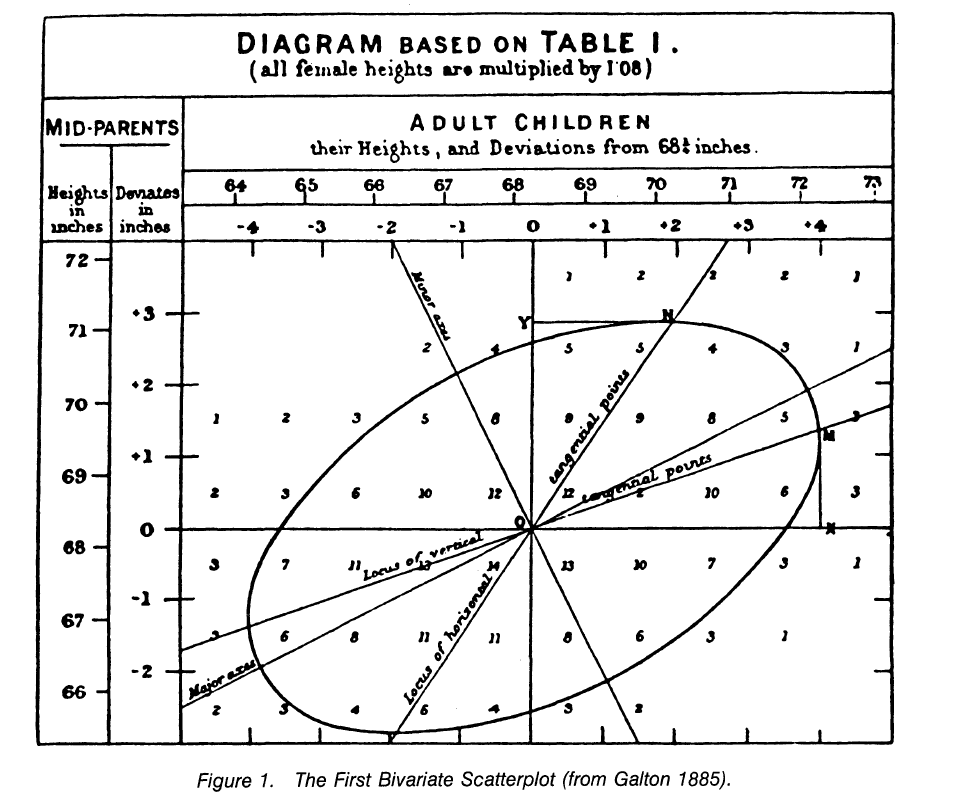
\includegraphics{galton.PNG}

\begin{itemize}
\tightlist
\item
  CORRELATION AS A FUNCTION OF RAW SCORES AND MEANS
\item
  CORRELATION AS STANDARDIZED COVARIANCE
\item
  CORRELATION AS THE GEOMETRIC MEAN THE TWO REGRESSION SLOPES
\item
  CORRELATION AS STANDARDIZED SLOPE OF THE REGRESSION LINE CORRELATION AS THE GEOMETRIC MEAN OF THE TWO REGRESSION SLOPES
\item
  CORRELATION AS THE SQUARE ROOT OF THE RATIO OF TWO VARIANCES (PROPORTION OF VARIABILITY ACCOUNTED FOR)
\item
  CORRELATION AS A FUNCTION OF THE ANGLE BETWEEN THE TWO STANDARDIZED REGRESSION LINES
\item
  CORRELATION AS A FUNCTION OF TEST STATISTICS FROM DESIGNED EXPERIMENTS
\item
  CORRELATION AS THE RATIO OF TWO MEANS
\item
  CORRELATION IN RELATION TO THE BIVARIATE ELLIPSES OF ISOCONCENTRATION
\item
  \ldots{}
\end{itemize}

\hypertarget{vizualization-of-covariance-and-correlation}{%
\chapter{Vizualization of covariance and correlation}\label{vizualization-of-covariance-and-correlation}}

\hypertarget{diffuxe9rentes-tentatives-pour-repruxe9senter-la-covariance}{%
\section{Différentes tentatives pour représenter la covariance}\label{diffuxe9rentes-tentatives-pour-repruxe9senter-la-covariance}}

\hypertarget{diagramme-de-venn}{%
\subsection{diagramme de Venn}\label{diagramme-de-venn}}

\begin{quote}
A Venn diagram is a widely used diagram style that shows the logical relation between sets, popularized by John Venn in the 1880s. The diagrams are used to teach elementary set theory, and to illustrate simple set relationships in probability, logic, statistics, linguistics and computer science. A Venn diagram uses simple closed curves drawn on a plane to represent sets. Very often, these curves are circles or ellipses.
\end{quote}

\emph{A compléter + insérer diagram}

\hypertarget{visualizing-distributions-of-covariance-matrices}{%
\subsection{Visualizing Distributions of Covariance Matrices}\label{visualizing-distributions-of-covariance-matrices}}

Covariance matrices and their corresponding distributions play an important role in statistics. To understand the properties of distributions, we often rely on visualization methods. \citep{VisCov}

But visualizing a distribution in a high-dimensional space is a challenge, with the additional
difficulty that covariance matrices must be positive semi-definite, a restriction that forces
the joint distribution of the covariances into an oddly-shaped subregion of the space.

\emph{je suis dépassé par cet article\ldots{}}

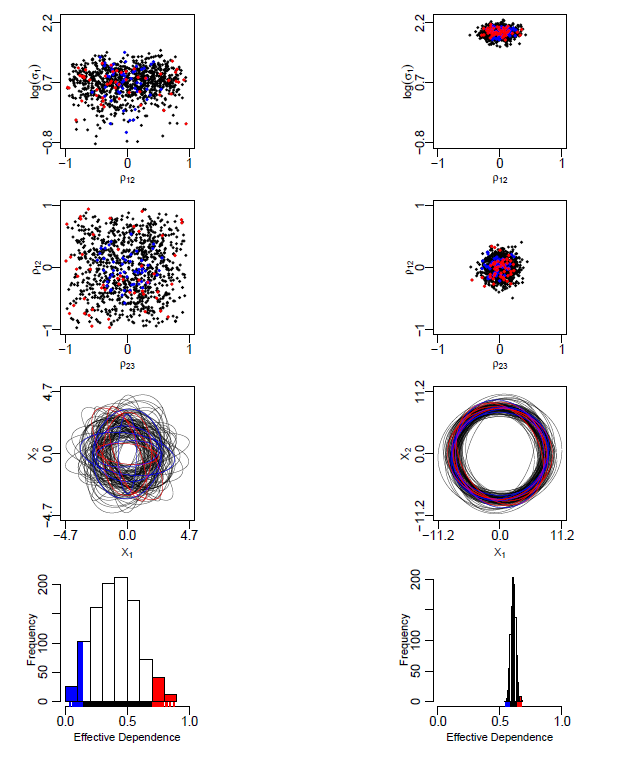
\includegraphics{wtf_covViz.PNG}

\hypertarget{visualization-of-covariance-and-cross-covariance-fields-uxe0-ne-pas-inclure}{%
\subsection{Visualization of covariance and cross-covariance fields (à ne pas inclure \ldots)}\label{visualization-of-covariance-and-cross-covariance-fields-uxe0-ne-pas-inclure}}

\emph{A étudier, qu'est ce que covariance fields exactement\ldots? } \citep{fields}

In mathematics, a field is a set on which addition, subtraction, multiplication, and division are defined and behave as the corresponding operations on rational and real numbers do. A field is thus a fundamental algebraic structure which is widely used in algebra, number theory, and many other areas of mathematics.

\emph{les schémas ont l'air intéressant mais les calculs et le sujet ont l'air trop complexes\ldots.}

\begin{quote}
In this paper, we present a numerical technique to visualize covariance and cross-covariance fields of two-dimensional stochastic simulation.
\end{quote}

\hypertarget{a-geometrical-interpretation-of-an-alternative-formula-for-the-sample-covariance}{%
\subsection{A Geometrical Interpretation of an Alternative Formula for the Sample Covariance}\label{a-geometrical-interpretation-of-an-alternative-formula-for-the-sample-covariance}}

Kevin Hayes \citep{Hayes} propose une nouvelle interprétation géométrique et visuelle de la covaraiance, à partir de l'application de la formule de la variance poposée par Hefferman. Il étend cette formule à la covariance d'un échantillon pour extraire ses résultats.

\begin{itemize}
\tightlist
\item
  formula from heffernan definition of covariance :
\end{itemize}

\[cov(X,Y)= \frac{2}{n(n-1)}\sum_{i=1}^{n-1}\sum_{j>i}^{n}\frac{1}{2}(x_i-x_j)(y_i - y_j)\]

Geometrically, \(\frac{1}{2}(x_i-x_j)(y_i - y_j)\) is ±1 times the area right-triangle formed with the difference vector \((x_i — x_j, y_j)\) as its hypotenuse, where negatively sloped difference tors incur a \((—1)\) sign and positively sloped difference vectors take a \((+1)\) sign. \citep{Hayes}

\textbf{\emph{A détailler et reformuler}}

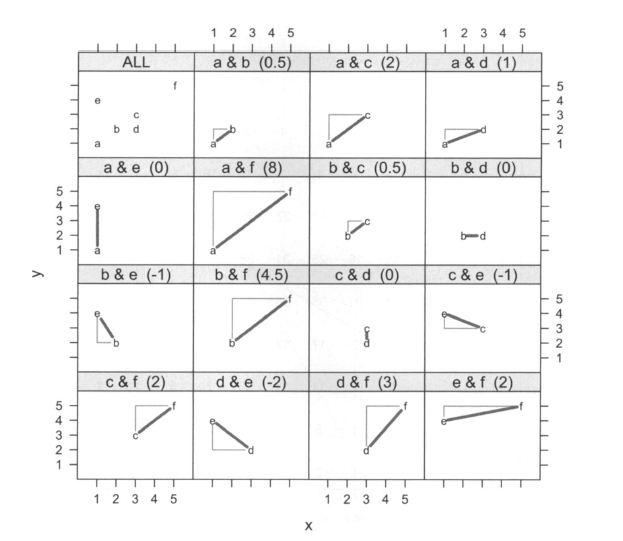
\includegraphics{hayes.PNG}

\hypertarget{covariance-as-signed-area-of-rectangles}{%
\subsection{Covariance as Signed Area of Rectangles}\label{covariance-as-signed-area-of-rectangles}}

Cet article \citep{chudzicki} a été écrit suite à une conversation trrès intéressante sur le site \textbf{stats.statckexchange} (\url{https://stats.stackexchange.com/questions/18058/how-would-you-explain-covariance-to-someone-who-understands-only-the-mean}.) Le sujet initial de cette conversation était : comment expliquer la covariance à quelqu'un qui ne comprends que la notion de moyenne?

mode d'emploi :

\begin{itemize}
\tightlist
\item
  Draw all possible such rectangles. Color them transparently, making the positive rectangles red (say) and the negative rectangles ``anti-red'' (blue).
\item
  The covariance is the net amount of red in the plot (treating blue as negative values).
\end{itemize}

Let's deduce some properties of covariance. Understanding of these properties will be accessible to anyone who has actually drawn a few of the rectangles. :

\begin{itemize}
\tightlist
\item
  Bilinearity.
\end{itemize}

Because the amount of red depends on the size of the plot, covariance is directly proportional to the scale on the x-axis and to the scale on the y-axis.

\begin{itemize}
\tightlist
\item
  Correlation.
\end{itemize}

Covariance increases as the points approximate an upward sloping line and decreases as the points approximate a downward sloping line. This is because in the former case most of the rectangles are positive and in the latter case, most are negative.

\begin{itemize}
\tightlist
\item
  Relationship to linear associations.
\end{itemize}

Because non-linear associations can create mixtures of positive and negative rectangles, they lead to unpredictable (and not very useful) covariances. Linear associations can be fully interpreted by means of the preceding two characterizations.

\begin{itemize}
\tightlist
\item
  Sensitivity to outliers.
\end{itemize}

A geometric outlier (one point standing away from the mass) will create many large rectangles in association with all the other points. It alone can create a net positive or negative amount of red in the overall picture.

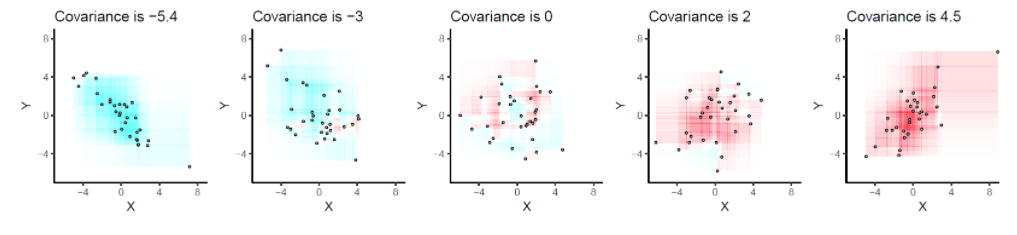
\includegraphics{covRect.PNG}

\hypertarget{covariance-and-regression-diagram}{%
\subsection{Covariance and regression diagram}\label{covariance-and-regression-diagram}}

Notre point de départ pour ce package est le travail réalisé par notre professeur \citep{bousquet}

\emph{schéma des différentes visualisations de la covariance}

\hypertarget{notre-projet-le-package-plotnetrec}{%
\section{Notre projet : le package plotnetrec}\label{notre-projet-le-package-plotnetrec}}

Une partie du package que nous en sommes en train de développer consiste à représenter la covariance.

\textbf{\emph{mettre schémas de représentation covariance issu de pltnetrec avec explications}}

\hypertarget{diagramme-de-ruxe9gression-et-repruxe9sentation-du-coefficient-de-duxe9termination}{%
\chapter{Diagramme de régression et représentation du coefficient de détermination}\label{diagramme-de-ruxe9gression-et-repruxe9sentation-du-coefficient-de-duxe9termination}}

\hypertarget{ols-deux-variables}{%
\section{OLS deux variables}\label{ols-deux-variables}}

\hypertarget{simple-linear-regression-model}{%
\subsection{simple linear regression model}\label{simple-linear-regression-model}}

\[y_i = \beta_0 + \beta_1x_i +  \epsilon_i\]
where \(\epsilon_i\) is te error or deviation of \(y_i\) from the line \(\beta_0 + \beta_1x_i\)

\begin{itemize}
\tightlist
\item
  Ordinary least square
\end{itemize}

We need to find the values of \(\beta_0\) and \(\beta_1\) that minimize the criterion :
\[S = \sum_{i=1}^n \epsilon_i^2 = \sum_{i=1}^n (y_i - (\beta_0 + \beta_1x_i))^2\]

Minimize this sum gives :

\[\hat{\beta_0}= \bar{y} - \hat{\beta_1}\bar{x}\]
\[\hat{\beta_1}= \frac{\sum_{i=1}^n(x_i -\bar{x})(y_i -\bar{y})}{\sum_{i=1}^n(x_i -\bar{x})^2}\]

\begin{itemize}
\tightlist
\item
  estimated simple linear regression model :
\end{itemize}

\[y_i = \hat{\beta_0} + \hat{\beta_1x_i} +  e_i\]

from which we can calculate a few additionnal quantities :

\begin{itemize}
\item
  \(\hat{y_i} = \hat{\beta_0} + \hat{\beta_1x_i}\) ; \(\hat{y_i}\) is the \textbf{predicted value} (or predicted fit) of y for the \(i^{th}\) observation in the sample.
\item
  \(e_i=y_i -\hat{y_i}\) ; is the \textbf{observed error} (or residual) for the \(i^{th}\) observation in the sample.
\item
  \(SSE = \sum_{i=1}^n (y_i -\hat{y_i})^2\) ; is the \textbf{sum of squared observed errors} for all observations in a sample of size \(n\)
\end{itemize}

\hypertarget{measuring-overall-variation-from-the-sample-line}{%
\subsection{Measuring overall variation from the sample line}\label{measuring-overall-variation-from-the-sample-line}}

\begin{itemize}
\item
  \(MSE = \frac{SSE}{n-p}\) , where \(p\) is the number of parametrers of the regression equation. \(p=2\) for regression with only one variable.
\item
  \(s = RMSE = \sqrt{(MSE)}\)
\item
  \(SSTO=\sum_{i=1}^n (y_i -\bar{y_i})^2\)
\item
  coefficient of determination :
\end{itemize}

\(R^2 = \frac{SSTO-SSE}{SSTO} = \frac{SSR}{SSTO}\) is the proportion of variation in \(y\) that is explained by \(x\).

c'est-à-dire que le coefficient de détermination est alors le rapport de la variance expliquée par la régression SSE sur la variance totale SST.

Le coefficient de détermination est le carré du coefficient de corrélation linéaire R entre les valeurs prédites \(\hat{y}_{i}\) et les mesures \(y_i\):

\[R^2=corr(\hat{y}_{i},y_i)\]

\(R^2\) does not indicate whether:

\begin{itemize}
\tightlist
\item
  the independent variables are a cause of the changes in the dependent variable;
\item
  omitted-variable bias exists;
\item
  the correct regression was used;
\item
  the most appropriate set of independent variables has been chosen;
\item
  there is collinearity present in the data on the explanatory variables;
\item
  the model might be improved by using transformed versions of the existing set of independent variables;
\item
  there are enough data points to make a solid conclusion.
\end{itemize}

\hypertarget{ols-3-variables}{%
\section{OLS 3 variables}\label{ols-3-variables}}

\hypertarget{ols-3-variables-et-plus}{%
\section{OLS 3 variables et plus}\label{ols-3-variables-et-plus}}

\hypertarget{reopruxe9sentation-de-la-ruxe9gression-linuxe9aire}{%
\chapter{Reoprésentation de la régression linéaire}\label{reopruxe9sentation-de-la-ruxe9gression-linuxe9aire}}

\hypertarget{etat-des-lieux-de-la-visualisation-de-la-ruxe9gression}{%
\section{Etat des lieux de la visualisation de la régression}\label{etat-des-lieux-de-la-visualisation-de-la-ruxe9gression}}

\hypertarget{more-on-venn-diagrams-for-regression}{%
\subsection{More on Venn Diagrams for Regression}\label{more-on-venn-diagrams-for-regression}}

Kennedy \citep{kennedy} extended the Venn diagram to the exposition of bias and variance in the context of the classical linear regression (CLR) model, written as y = Xb + e .

\emph{A compléter}

\hypertarget{a-geometric-approach-to-compare-variables-in-a-regression-model}{%
\subsection{A Geometric Approach to Compare Variables in a Regression Model}\label{a-geometric-approach-to-compare-variables-in-a-regression-model}}

He proposes \citep{Bring} a geometric approaches to compare variables in a regression model.

\begin{quote}
This article gives a brief introduction to the geometric approach in regres- sion analysis, and then geometry is used to shed some light on the problem of comparing the ``importance'' of the in- dependent variables in a multiple regression model. Even though no final answer of how to assess variable impor- tance is given, it is still useful to illustrate the different measures geometrically to gain a better understanding of their properties.
\end{quote}

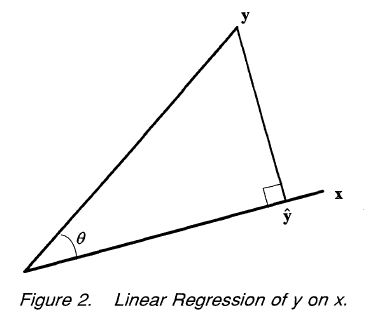
\includegraphics{bring1.PNG}

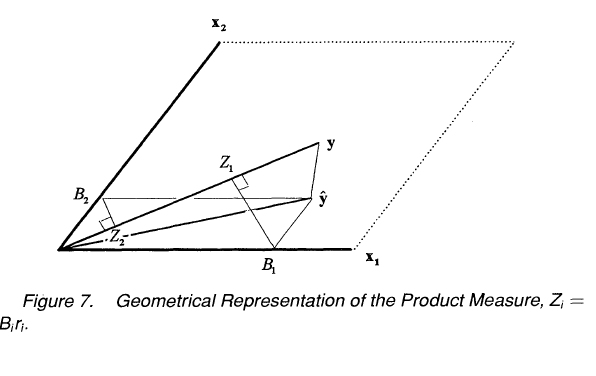
\includegraphics{bring.PNG}

\emph{A compléter}

\hypertarget{two-additional-views-of-linear-regression-coefficients}{%
\subsection{Two Additional Views of Linear Regression Coefficients}\label{two-additional-views-of-linear-regression-coefficients}}

The author \citep{Cli} proposes an interesting interpretation of the slope in the keast square method. The linear regression line of y on x, as determined by the method of least squares, passes through the central point with slope:

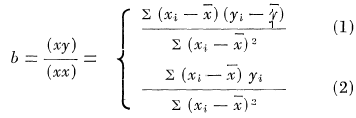
\includegraphics{slope.PNG}

\begin{itemize}
\tightlist
\item
  As a weighted average slope.
\end{itemize}

\begin{quote}
This concept of weight for a slope is represented in the accompanying diagrams. (See Figure 1). The slope in the lefthand side diagram has a much larger weight than that in the righthand side for regression of y on x. If we were concerned with the regression of x on y, the reverse would be true. Note that the actual distance between the two points in the two diagrams is the same.
\end{quote}

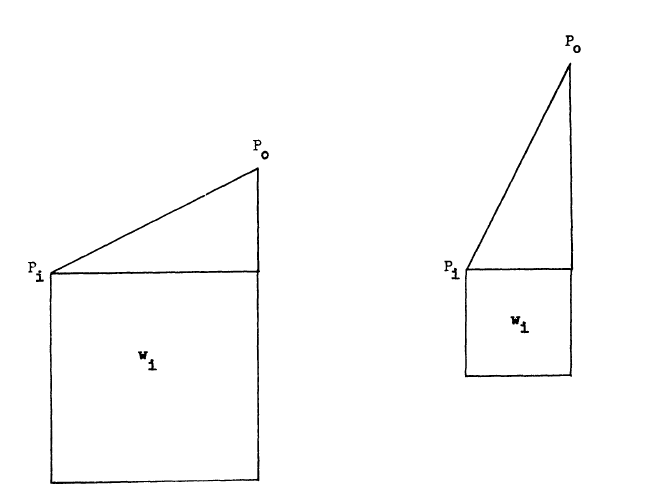
\includegraphics{LI_slope.PNG}

\begin{itemize}
\tightlist
\item
  As a contrast
\end{itemize}

*A détailler \ldots{} ou pas \ldots{}

\hypertarget{covariance-and-regression-diagram-1}{%
\subsection{Covariance and regression diagram}\label{covariance-and-regression-diagram-1}}

Notre point de départ pour ce package est le travail réalisé par notre professeur \citep{bousquet}

\emph{schémas LS à insérer}

\hypertarget{notre-projet-le-package-plotnetrec-1}{%
\section{Notre projet: le package plotnetrec}\label{notre-projet-le-package-plotnetrec-1}}

\hypertarget{etat-des-lieux-des-package-r-en-uxe9conomuxe9trie-de-la-visualisation}{%
\chapter{Etat des lieux des package R en économétrie de la visualisation}\label{etat-des-lieux-des-package-r-en-uxe9conomuxe9trie-de-la-visualisation}}

\begin{itemize}
\tightlist
\item
  viscov
\end{itemize}

Our visualizations follow the principle of decomposing a covariance matrix into scale parameters and correlations, pulling out marginal summaries where possible and using two and three-dimensional plots to reveal multivariate structure. Visualizing a distribution of covariance matrices is a step beyond visualizing a single covariance matrix or a single multivariate dataset.

\begin{itemize}
\tightlist
\item
  Colourpicker
\end{itemize}

Colourpicker is a tool for Shiny framework and for selecting colours in plots. This tool supports various options, such as alpha opacity, custom colour palettes, and more. The most common uses of this tool include the utilisation of the colourInput() function to create a colour input in Shiny as well as the use of the plotHelper() function/RStudio Addin to select colours for a plot.

\begin{itemize}
\tightlist
\item
  Esquisse
\end{itemize}

The esquisse package allows a user to interactively explore data by visualising it with the ggplot2 package. It allows a user to draw bar graphs, curves, scatter plots, histograms, export the graphs, and retrieve the code generating the graph. With the help of esquisse, one can quickly visualise the data according to their type as well as export to PNG or PowerPoint, and retrieve the code to reproduce the chart.

\begin{itemize}
\tightlist
\item
  ggplot2
\end{itemize}

ggplot is a popular package that is based on the grammar of graphics. The idea behind this library is that one can build every graph from the same components, such as a dataset, a coordinate system, and more. The package provides graphics language for creating intuitive and intricate plots. It allows a user to create graphs that represent both univariate and multivariate numerical and categorical data.

\begin{itemize}
\tightlist
\item
  ggvis
\end{itemize}

ggvis is a data visualisation package for R that allows to declaratively describe data graphics with a syntax similar in spirit to ggplot2. It allows creating rich interactive graphics locally in Rstudio or in the browser as well as leverage the infrastructure of the Shiny package to publish interactive graphics usable from any browser. The goal of ggvis is to make it easy to build interactive graphics for exploratory data analysis.

\begin{itemize}
\tightlist
\item
  ggforce
\end{itemize}

The ggforce is a package aimed at providing missing functionality to ggplot2 through the extension system introduced with ggplot2 v2.0.0. The goal of this package is to provide a repository of geoms, stats, among others. Using ggforce, one can enhance almost any ggplot by highlighting data groupings and focusing attention on interesting features of the plot.

\begin{itemize}
\tightlist
\item
  lattice
\end{itemize}

Lattice is a powerful high-level data visualisation system for R that is designed with an emphasis on multivariate data and allows to create multiple small plots easily. The lattice package attempts to improve on base R graphics by providing better defaults and the ability to display multivariate relationships easily. Particularly, the package supports the creation of trellis graphs that show a variable or the relationship between variables, conditioned on one or more other variables.

\begin{itemize}
\tightlist
\item
  Plotly
\end{itemize}

Plotly is an open-source R package for creating interactive web-based graphs via the open-source JavaScript graphing library plotly.js. The Plotly's R graphing library helps in creating interactive, publication-quality graphs including line plots, scatter plots, area charts, bar charts, error bars, etc. One can use Plotly for R to make, view and distribute charts and maps online as well as offline.

\begin{itemize}
\tightlist
\item
  patchwork
\end{itemize}

patchwork is a package that expands the API to allow for the arbitrarily complex composition of plots by providing mathematical operators for combining multiple plots. The goal of patchwork is to make it simple to incorporate separate ggplots into the same graphic.

\begin{itemize}
\tightlist
\item
  quantmod
\end{itemize}

quantmod is an R package that provides a framework for quantitative financial modelling and trading. It provides a rapid prototyping environment that makes modelling easier by removing the repetitive workflow issues surrounding data management and visualisation.

\begin{itemize}
\tightlist
\item
  RGL
\end{itemize}

The RGL package is used to produce interactive 3-D plots using OpenGL. The library contains high-level graphics commands modelled loosely after classic R graphics and working in three dimensions. It also includes a low-level structure inspired by the grid package. RGL provides medium to high-level functions for 3D interactive graphics, including functions modelled on base graphics as well as functions for constructing representations of geometric objects.

\begin{itemize}
\tightlist
\item
  Highcharter
\end{itemize}

is an R wrapper for Highcharts, an interactive visualization library in JavaScript. Like its predecessor, highcharter features a powerful API.

Highcharter makes dynamic charting easy. It uses a single function, hchart(), to draw plots for all kinds of R object classes, from data frame to dendrogram to phylo. It also gives R coders a handy way to access the other popular Highcharts plot types, Highstock (for financial charting) and Highmaps (for schematic maps in web-based projects).

\begin{itemize}
\tightlist
\item
  Leaflet
\end{itemize}

Like highcharter, Leaflet for R is another charting packaged based on a hugely-popular JavaScript library of the same name.

Leaflet offers a lightweight but powerful way to build interactive maps, which you've probably seen in action (in their JS form) on sites ranging from The New York Times and The Washington Post to GitHub and GIS specialists like Mapbox and CartoDB.

The R interface for Leaflet was developed using the htmlwidgets framework, which makes it easy to control and integrate Leaflet maps right in R Markdown documents (v2), RStudio, or Shiny apps.

\begin{itemize}
\tightlist
\item
  RcolorBrewer
\end{itemize}

RColorBrewer makes it easy to take advantage of one of R's great strengths: manipulating colors in plots, graphs, and maps.

The package is based on Cynthia Brewer's work on the use of color in cartography (check out Colorbrewer to learn more), and it lets you create nice-looking sequential, diverging, or qualitative color palettes. It also plays nicely with Plotly, as these examples by Plotly demonstrate.

\begin{itemize}
\tightlist
\item
  dygraphs
\end{itemize}

This package provides an R interface for dygraphs, a fast, flexible JavaScript charting library for exploring time-series data sets. What's powerful about dygraphs is that it's interactive right out of the box, with default mouse-over labels, zooming, and panning. It's got lots of nifty other interactivity features, like synchronization or the range selector shown above.

But dygraph's interactivity doesn't come at the expense of speed: it can handle huge datasets with millions of points without slowing its roll. And you can use RColorBrewer with dygraphs to choose a different color palette for your time series--- check out this example to see how.

\begin{itemize}
\tightlist
\item
  sunburst
\end{itemize}

pas forcément utile pour notre sujet

\begin{itemize}
\tightlist
\item
  VennDiagram
\end{itemize}

Create a Venn diagram and save it into a file. The function venn.diagram() takes a list and creates a file containing a publication-quality Venn Diagram.

  \bibliography{references.bib}

\end{document}
